% \begin{figure*}[ht]
%     \centering
%     \begin{subfigure}{.5\textwidth}
%       \centering
%       \includegraphics[width=.8\linewidth]{figures/60.png}
%       \caption{$T_{prl} = 60s$}
%     \end{subfigure}%
%     \begin{subfigure}{.5\textwidth}
%       \centering
%       \includegraphics[width=.8\linewidth]{figures/300.png}
%       \caption{$T_{prl} = 300s$}
%     \end{subfigure}
%     \caption{Results of our simulation on the evolution of the \ac{PRL} size
%     over time, each second revoking a pseudonym non-deterministically with
%     probability 0.1. After an initial growth, the number of elements in the list
%     fluctuates around $T_{prl} * 0.1$.}
%     \label{fig:eval-prl-size}
% \end{figure*}


% Adjustments to auto generated plot:
% 1 to axis add 
% width=\columnwidth,
% legend pos=north west,
% xticklabel style = {
%       /pgf/number format/fixed,
%       /pgf/number format/precision=6
%   },
% scaled x ticks=false,
% T_PRL = 300
% n=400
% 

\begin{figure}[t]
\centering
% This file was created with tikzplotlib v0.10.1.
% This file was created with tikzplotlib v0.10.1.
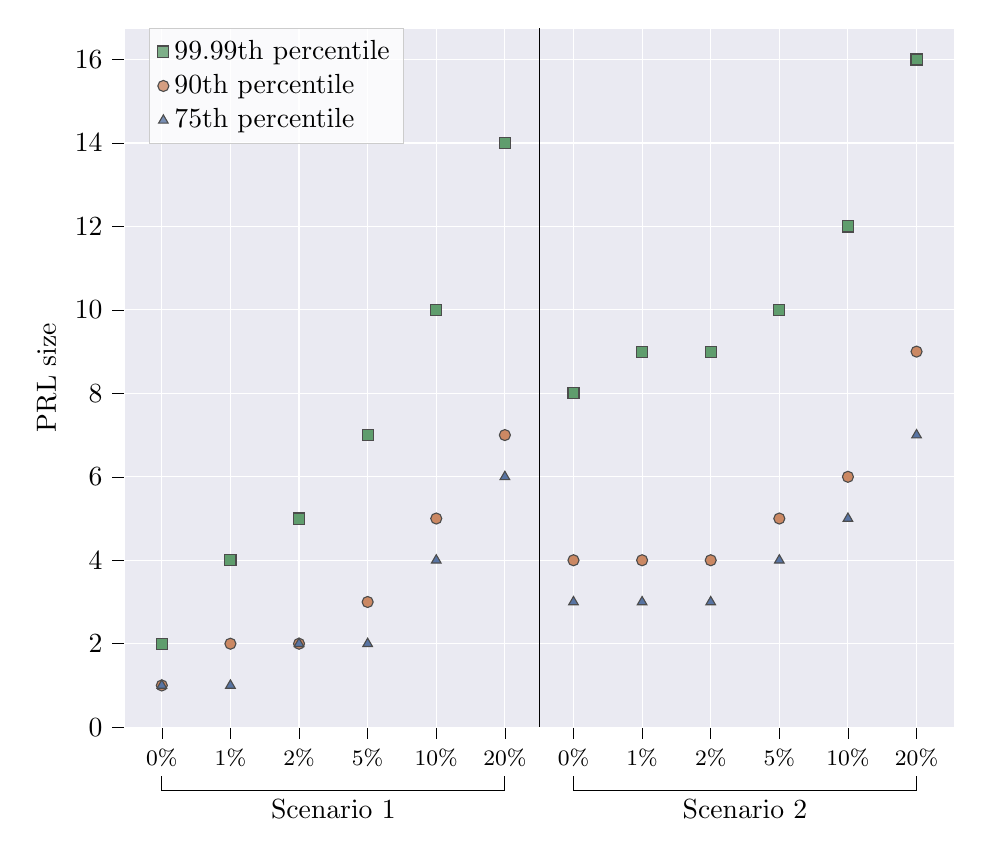
\begin{tikzpicture}

  \definecolor{lightgray204}{RGB}{204,204,204}
  \definecolor{darkslategray38}{RGB}{38,38,38}
  \definecolor{darkslategray76}{RGB}{76,76,76}
  \definecolor{indianred1819295}{RGB}{181,92,95}
  \definecolor{lavender234234242}{RGB}{234,234,242}
  \definecolor{lightslategray133122170}{RGB}{133,122,170}
  \definecolor{mediumseagreen95157109}{RGB}{95,157,109}
  \definecolor{peru20313699}{RGB}{203,136,99}
  \definecolor{steelblue76114176}{RGB}{76,114,176}
  \definecolor{steelblue88116163}{RGB}{88,116,163}
  
  \begin{axis}[
    width=\columnwidth,
    ylabel= PRL size,
    xmajorgrids,
    xmajorticks=true,
    ymajorgrids,
    ymajorticks=true,
    axis background/.style={fill=lavender234234242},
    axis line style={white},
    x grid style={white},
    y grid style={white},
  legend cell align={left},
  legend style={
    fill opacity=0.8,
    draw opacity=1,
    text opacity=1,
    at={(0.03,1.0)},
    anchor=north west,
    draw=lightgray204
  },
  tick align=outside,
  tick pos=left,
  % x grid style={darkgray176},
  xmin=-0.55, xmax=11.55,
  xtick style={color=black},
  xtick={0,1,2,3,4,5,6,7,8,9,10,11},
  xticklabel style={name=tick no \ticknum, font=\footnotesize},
  xticklabels={
    $0\%$,
    $1\%$,
    $2\%$,
    $5\%$,
    $10\%$,
    $20\%$,
    $0\%$,
    $1\%$,
    $2\%$,
    $5\%$,
    $10\%$,
    $20\%$
  },
  % y grid style={darkgray176},
  ymin=0.0, ymax=16.75,
  ytick style={color=black}
  ]
  \addplot [draw=darkslategray76, fill=mediumseagreen95157109, mark=square*, only marks]
  table{%
x  y
0 2
1 4
2 5
3 7
4 10
5 14
6 8
7 9
8 9
9 10
10 12
11 16
};
\addlegendentry{99.99th percentile}
\addplot [draw=darkslategray76, fill=peru20313699, mark=*, only marks]
table{%
x  y
0 1
1 2
2 2
3 3
4 5
5 7
6 4
7 4
8 4
9 5
10 6
11 9
};
\addlegendentry{90th percentile}
\addplot [draw=darkslategray76, fill=steelblue88116163, mark=triangle*, only marks]
table{%
x  y
0 1
1 1
2 2
3 2
4 4
5 6
6 3
7 3
8 3
9 4
10 5
11 7
};
\addlegendentry{75th percentile}

\draw (axis cs:5.5,0) -- (axis cs:5.5,45);

% \draw (axis cs:0.0, -2) -- (axis cs:0.0, -4) -- (axis cs:5.0, -4) -- (axis cs:5.0, -2);


\end{axis}
\draw  (tick no 0.south) -- +(0,-.5em) -- ([yshift=-.5em] tick no 5.south)  node [midway, below] {Scenario 1}  -- +(0,.5em);
\draw  (tick no 6.south) -- +(0,-.5em) -- ([yshift=-.5em] tick no 11.south) node [midway, below] {Scenario 2} -- +(0,.5em);
  
  \end{tikzpicture}
  
\caption{Markov model percentiles for maximum PRL sizes for $T_{prl}=30s$,
  $n=800$, and different shares of attackers in each baseline revocation
  scenario.}
\label{fig:eval-prl-size}
\end{figure}
